\begin{center}
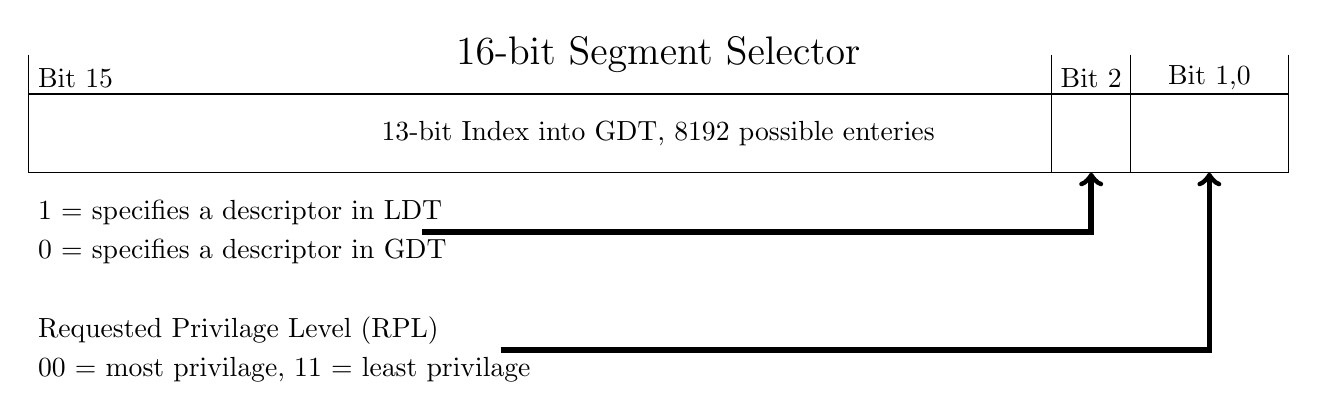
\begin{tikzpicture}
\draw node at (8,1.5) {{\Large 16-bit Segment Selector}};
\draw (0,0)  rectangle (16,1) node [pos=0.5] {13-bit Index into GDT, 8192 possible enteries};
\foreach \x in {16,14,13,0}
\draw (\x,1.5) -- (\x,0);
\draw node at (15,1.2) {Bit 1,0};
\draw node at (13.5,1.2) {Bit 2};
\draw node at (0,1.2) [right] {Bit 15};
\draw node at (0,-0.5) [right] {1 = specifies a descriptor in LDT};
\draw node at (0,-1) [right] {0 = specifies a descriptor in GDT};
\draw node at (0,-2) [right] {Requested Privilage Level (RPL)};
\draw node at (0,-2.5) [right] {00 = most privilage, 11 = least privilage};
\draw[->, line width = 2pt] (5,-0.75) -- (13.5,-0.75) -- (13.5,0);
\draw[->, line width = 2pt] (6,-2.25) -- (15,-2.25) -- (15,0);
\end{tikzpicture}
\end{center}